\documentclass[main.tex]{subfiles}
\begin{document}
\section{Neutron Tagging with the Analog Setup}
\subsection{Energy Calibrated NE213 QDC Spectrum}
Each particle interacting in the detector will leave a footprint in the form of a pulse of charge. In the analog setup we use charge to digital converters to parameterize these pulses into measures of the deposited energy. Pulses are integrated on two different timescales: 60 and 500 nanoseconds. Together they can be used to express the pulse shape, PS, through the fraction of charge located in the tail. This parameter is unitless, but it is still of interest to convert the total integrated charge from units of QDC channels to some measure of energy.

In the NE213 detector neutrons interact via the strong force with nuclei while gammas primarily interacts via the electromagnetic force with atomic electrons. This means that the pulses they produce in the detector originate from entirely different particles and processes, and consequently we can not callibrate our spectrum in terms of the particles kinetic energy. Instead we calibrate it in terms of the electron equivalent energy. That is the energy an electron would need to have had in order to produce the same integrated charge in the detector.

During one hour of measurements 4.3 million events were recorded by the analog setup. Because the QDC baseline has been known to occasionally drift by tens of channels during acquisition it was necessary to to observe and compensate for any drift. By allowing the acquisition start to trigger on YAP signals as well as NE213 signals a large amount of windows with no signals were integrated. These events represent the vaseline offset. The number of YAP signals sent to the trigger was reduced by a factor of 256 with a prescaler. However, during this particular data acquisition the pedestal remained stationary.

\begin{table}[hb]
	\center
	\begin{tabular}{|l|l|l|l|}
	\hline
	ADC             & 67.5 & 11.43 & 2718 \\
	\hline
	E(MeV)          & 0    & 2.23  & 4.44 \\
	\hline
	$(E_{e})_{max}(MeV_{ee})$ & 0    & 2.00  & 4.20 \\
	\hline
	\end{tabular}
	\label{tab:knox}
   	\captionsetup{width=0.435\linewidth}
	\caption{Table of ADC values and the corresponding energies. See text for details.}
\end{table}

The uncalibrated QDC spectrum is shown in fig \ref{fig:qdc_a} top panel. The narrow peak located to the far left is the pedestal. It is produced when a YAP trigger gives a start signal causing the QDC module to integrate only the baseline. The bump immediately to the right of it is produced when this YAP trigger actually coincides with something. This may be the case when the gamma interacting in the YAP was produced together with a neutron or another gamma ray or when it scatters from the YAP and into NE213 detector.

The 2.23 and the 4.4 MeV Compton edges have been highlighted in green and red. Using the Knox method a set of points corelating the energy deposition in ADC channels to $MeV_{ee}$. The points are also shown in table \ref{tab:knox}. Using these points a linear fit was madeand plotted in in fig \ref{fig:qdc_a} middle panel. The fit does not pass through the points so nicely, but does nearly pass through zero.

using this fit the QDC spectrum was converted to $MeV_{ee}$. The calibrated energy spectrum is shown in the bottom panel of fig \ref{fig:qdc_a}.
\begin{figure}[ht!]
    \centering
        \includegraphics{AnalogResults/Ecall.pdf}
        \caption{Top: The raw QDC spectrum. Middle: The callibration fit produced with the Knox method. Bottom: The energy calibrated QDC spectrum.}
    \label{fig:qdc_a}
\end{figure}
\clearpage
\subsection{Pulse Shape Discrimination}
Since neutrons and gammas interact differently in the NE213 detector their signal have different shape and duration. This makes it possible to discriminate between neutrons and gammas. The pulses were integrated over 500 ns and 60 ns and a constant 120 QDC channels was added to the shortgate QDC values, in order to linearize the pulse shape as a function of deposited energy. This corresponds to shifting the baseline of the signals during shortgate integration. No constant was added to the longgate QDC values. The pedestal events were not of interest for pulse shape discrimination,  so only events above 0.8 $MeV_{ee}$ deposited energy were used. As can be seen from fig \ref{fig:qdc_a} there is some overlap between pedestal events and the PuBe energy spectrum. This will be addressed when we look at the time of flight.

The resulting spectrum is shown in fig \ref{fig:psd_a}. The upper band is made up of pulses for which the tail contained a relatively large amount of the charge. This is the neutron band. Conversely The lower is made up of gammas for which most of the energy is carried in the body of the pulse. 

\begin{figure}[ht]
    \centering
        \includegraphics{AnalogResults/psd.pdf}
        \caption{Heatmap of the fraction of total integrated charge as a function of energy. The dashed white line indicates the discrimination cut (tail/total = 0.259).}
        \label{fig:psd_a}
\end{figure}
The analog setup applies an amplitude threshold of 100 mV. Since neutrons have more charge in the tail a 100 mV amplitude neutron signal can be expected to deposit more energy in the detector than a 100 mV amplitude gamma pulse. This gives rise to the curved energy threshold we see in the figure. It is also noteable that the neutron band seems to be one single distribution, whereas the gamma band has two clear peaks. This is because the neutrons are produced with a continuous distribution of energies whereas the gammas are produced with specific energies in the deexcitation of nuclei.

The linearization made it possible to draw a straight line through the spectrum, which separates neutrons from gammas. The procedure by which this cut was determined will be presented in parallel for the digital and the analog setup in chapter \ref{sec:results}. For now we just note that PS=0.259, shown as a dashed line in fig \ref{fig:psd_a}, was found to provide the best spearation. Seeing how the neutron and gamma distributions seem to overlap at low energies this cut will likely cause some misclassification. Studying the time of flight can help us to get an idea of the extent of this misclassification.


\subsection{Time of Flight spectrum}
By correlating signals in the NE213 detector with those in the YAP we can tag neutrons and gammas in order to construct a time of flight spectrum. For practical reasons NE213 signals are used as start signals for the TDC while the gamma signals are delayed and used as stop signals. Thus the raw time of flight spectrum will contain a neutron peak to the left of a gamma peak. In fig \ref{fig:tof_a} this has been accounted for by switching the sign, converting from TDC channels to nanoseconds using the time calibration factor found in chapter \ref{sec:exp_setup}, and shifting the gamma peak to time $t=10cm/c$ (the approximate time it takes light to reach the YAP detector). 

Since all the gammas travel at the speed of light one might expect a much narrower gamma peak. The are a number of reasons why this is not the case. First of all the gamma source and the detectors all have some size, so there are multiple paths light can take from source to detector. Secondly interactions are stochastic, so each gamma will travel some distance into a detector before interacting, which is particularly relevant for the much larger NE213 detector. The distance travelled through cables and the various electronic components, will also cause some attenuation, which may lead to differences in risetime of low and high amplitude pulses. This will in turn make the constant fraction discriminator less effective causing some loss in the time resolution. Furthermore, the final  digitization by the TDCs may cause some loss of resolution.

Since the distance from source to detector is known we can convert the neutron time of flight into Energy. The insert in fig \ref{fig:A_TOF} shows the energy of particles located in the neutron peak, with higher flight times maps to lower energies. The interval used is highlighted by the red dotted lines.
\begin{figure}[ht]
    \centering
        \includegraphics{AnalogResults/tof.pdf}
        \caption{The time calibrated time of flight spectrum. The x-axis denotes the time of flight from source to NE213 detector. The neutron and gamma peaks have been indicated with arrows and the upper right insert shows the energy distribution of events located in the neutron peak}
    \label{fig:tof_a}
\end{figure}

With time of flight information in hand we have a powerful tool for revisiting the energy cut made to separate out the pedestal events as well as the pulse shape discrimination cut. Figure \ref{fig:tof_ps_a} shows pulse shape as a function of time of flight, with neutron and gamma distributions highlighted. It is clear that it is not possible to make a discrimination cut on the pulse shape parameter without significant misclassification. 

Often the start and stop signal will be due to random coincidences. On small timescales of a few hundred nanoseconds these events are expected to form a flat background in the time of flight spectrum. Since These events still represent either neutrons or gammas one would expect them to be separated into two bands in \ref{fig:tof_ps_a}. One above and one below the cut. However the distributions are not far enough from one another for this to be visible.
Another interesting feature is that there is large amount of gammas at higher energies. This is because not all pedestal events were remove by the cut at 0.8 MeV and these events use the same signal as start and stop, so these will appear to be simultaneous. The reason why they appear to have such high fraction of tail/total must be that signal delays cause the integration to occur on the tail of pulses.
\begin{figure}[ht]
    \centering
        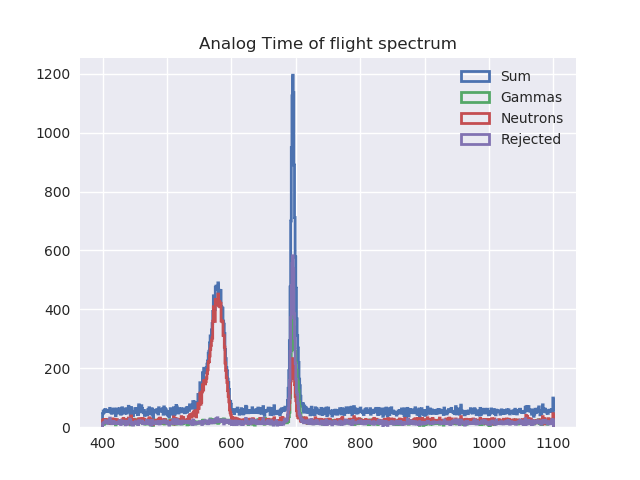
\includegraphics{AnalogResults/tof_psd.pdf}
        \caption{Time of flight plotted against fraction of charge located in the tail of signals. The dashed white line indicates the discrimination cut at tail/total = 0.259. A logarithmic z-axis is used to highlight the distribution of background events. Pedestal events have been removed with a cut at 0.8 $MeV{ee}$.}
    \label{fig:tof_ps_a} 
\end{figure}

We can gain some more information on the effect of the injected pedestal events by looking at \ref{fig:tof_E}. Above 0.8 $MeV{ee}$ We have a gamma and a neutron destribution as marked by the arrows. As expected gamma time of flight is independent of energy deposition. It is also clear that the pedestal events mostly land at the gamma time of flight. This is to be expected since these signals are acting as both start and stop signals. It is also clear that the cut at 0.8 $MeV{ee}$ will not be able to remove all of the pedestal. Unlike the gamma flash the neutron distribution show some correlation between time of flight and energy deposition. It seems that the faster neutrons are able to deposit more energy than the slower ones.

In fig \ref{fig:tof_Edep_Eneutron_a} the deposited energy is shown as a function of neutron kinetic energy as ffound from the time of flight spectrum. It can be seen that high energy deposition implies high neutron energy. However, the converse is not necessarily true as neutrons may scatter out of the detector before depositing their maximum energy. It is interesting that the energy the detector sees in $MeV_{ee}$ appears to be only half of the neutrons kinetic energy in  $MeV$.

\begin{figure}[ht]
    \centering
        \includegraphics{AnalogResults/tof_E.pdf}
        \caption{Time of flight plotted against energy deposition.}
    \label{fig:tof_E_a} 
\end{figure}

\begin{figure}[ht]
    \centering
        \includegraphics{AnalogResults/tof_Edep_Eneutron.pdf}
        \caption{Neutron energy as a function of deposited energy in the NE213 detector.}
    \label{fig:tof_Edep_Eneutron_a} 
\end{figure}




\end{document}
